
\begin{frame}{The Margin Is Pre-Trend Clean; Turnout and Valid Votes Are Not}
\hypertarget{src:pretrend}{}
\small
A free 2016 lag raises a fair question: does the instrument load on municipalities already moving in the consolidating direction? To test this we regress the 2016$\to$2020 pre-period change on the instrument, conditioning only on pre-determined (2010 Census) covariates and state FE. A clean, share-exogenous design wants every coefficient near zero, since the shock should not predict past movement.
\smallskip
\begin{center}
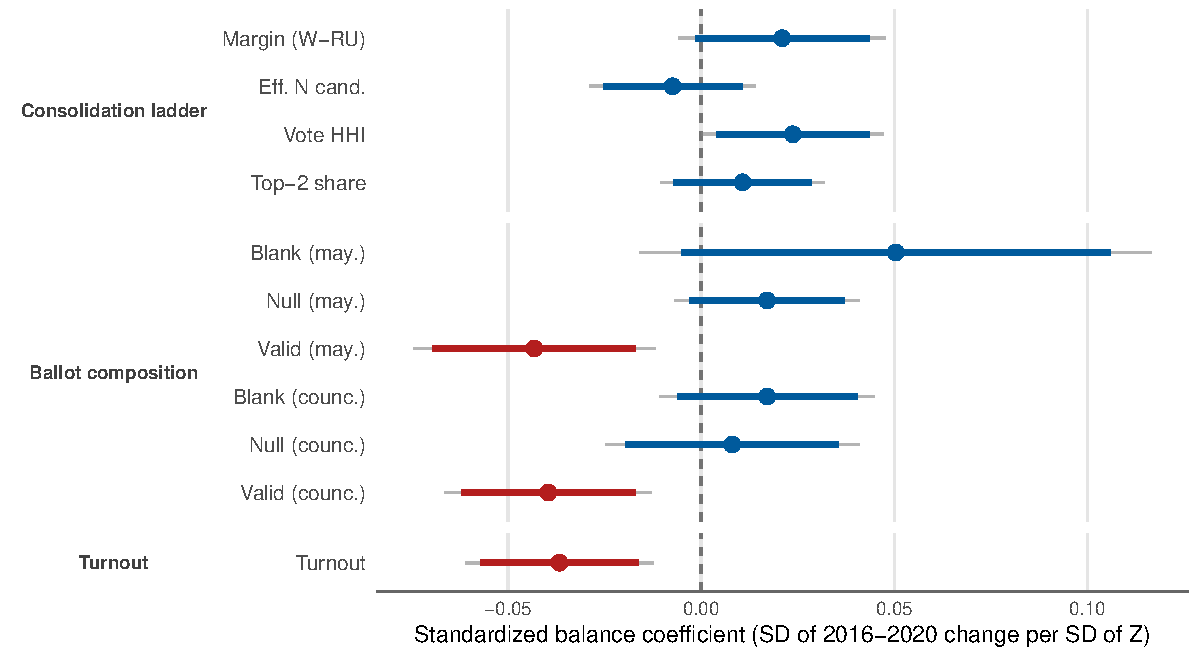
\includegraphics[width=\linewidth,height=0.44\textheight,keepaspectratio]{../figures/pretrend_coefplot.pdf}
\end{center}
\smallskip
\footnotesize Margin ($p=\PtRFMarginP$), effective-N ($p=\PtRFEffNP$) and top-two share ($p=\PtRFTopTwoP$) are clean; the Herfindahl is borderline ($p=\PtRFHHIP$, and tF rejects on the 2SLS placebo). Mayoral blank ($p=\PtRFBlankP$) and null ($p=\PtRFNullP$) are clean. \PtNFail{} of \PtNTests{} tests fail at 5\%: turnout ($p=\PtRFTurnoutP$), the mayoral valid rate ($p=\PtRFValidP$) and the council valid rate ($p=\PtRFValidVerP$). By seat, the margin pre-trends in open seats ($\OpenPtMarginCoef$, $p=\OpenPtMarginP$) and not in contested ones ($p=\ContPtMarginP$). Adding the 2020 level as a second lag moves the margin from $\MarginCoef$ to $\PtRobMarginCoef$ ($p=\PtRobMarginP$) \hyperlink{app:ptrobust}{\beamergotobutton{full pre-path}}. \emph{(Thick 90\%, thin 95\% CI; red $p<.05$.)}\hfill\hyperlink{app:pretrend}{\beamergotobutton{Placebo table}}
\end{frame}
